\documentclass{scrartcl}
\usepackage{etex}
\usepackage[ngerman]{babel}
\usepackage[utf8]{inputenc}
\usepackage[T1]{fontenc}
\usepackage{amsmath, amssymb}
\usepackage{graphicx}

\usepackage{pgfplots}
\pgfplotsset{compat=1.11}
\usepgfplotslibrary{external}
\usepackage{pgfplotstable}

\usepackage{booktabs}
\usepackage{multirow}
\usepackage{longtable}
\usepackage{ulsy}
%\usepackage{pst-all}
\usepackage{picture}
\usepackage[automark]{scrpage2}
\usepackage{caption}
\pagestyle{scrheadings}
\ihead[]{Friedrich Hübner 2897111}
\ohead[]{Fiona Paulus 2909625} 

\author{Friedrich Hübner 2897111\\
Fiona Paulus 2909625}
\title{Computerphysik\\Hausarbeit 2}

\begin{document}
\maketitle
\newpage

\section*{Allgemeine Hinweise}
Das Programm wurde unter Windows 10 mit "g++ -o abgabe2.exe -Wall -Wextra -std=c++0x -O2 -static abgabe2.cpp"\;kompiliert.\\
Das Programm wird gestartet mit 'abgabe2 a V0', wobei a in pm und V0 in eV ist. 

\section*{Aufgabe 1}
Da $z = q \cdot a$ und sowohl $q\geq 0$ als auch $a > 0$ folgt: $z \geq 0$.\\
Weiterhin wird $q$ maximal bei $E = 0$ mit $z_{max} = a q_{max} = a\frac{\sqrt{2m_eV_0}}{\bar{\hslash}} = \xi$. Also ist $0 \leq z \leq \xi$.

\section*{Aufgabe 2}
Da $\frac{\sqrt{\xi^2-z^2}}{z} \geq 0$ müssen auch $\tan z$ bzw. $-\cot z$ positiv sein. Der Tangens ist nicht-negativ auf den Intervallen $[k\pi, k\pi+\frac{\pi}{2})$, der negative Cotangens auf $[k\pi+\frac{\pi}{2}, (k+1)\pi), k \in \mathbb{Z}$.\\
Auf den angegebenen Intervallen sind beide Funktionen auch stetig und streng monoton steigend: $\tan' z = \frac{1}{\cos^2 z} > 0$, $-\cot' z = \frac{1}{\sin^2 z} > 0$.\\
Weiterhin ist $\frac{\sqrt{\xi^2-z^2}}{z}' = -\cfrac{z\sqrt{\xi^2-z^2} + \frac{z}{\sqrt{\xi^2-z^2}}}{\xi^2-z^2} < 0$ und somit ist $\frac{\sqrt{\xi^2-z^2}}{z}$ streng monoton fallend.\\

\subsection*{gerader Fall: $g(z) = \tan z - \frac{\sqrt{\xi^2-z^2}}{z}$}

\begin{center}
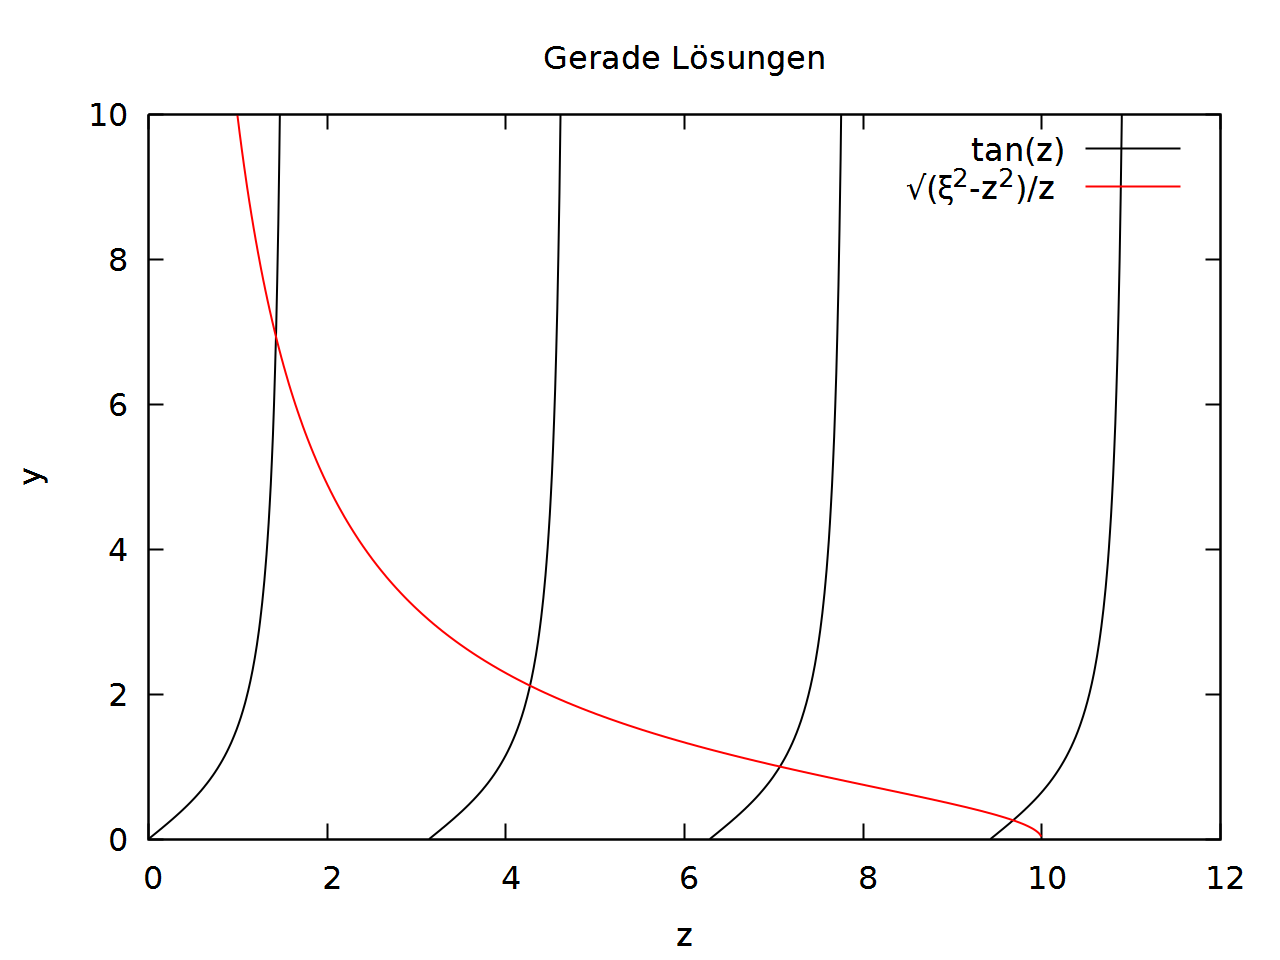
\includegraphics[scale=0.3]{plot_tan.png}
\captionof{figure}{Gerader Fall $\xi = 10$}
\end{center}

In dem Diagramm wurden sowohl $\tan z$ als auch $\frac{\sqrt{\xi^2-z^2}}{z}$ eingezeichnet. Jeder Schnittpunkt entspricht einer Lösung. Wie man gut erkennen kann, gibt es auf jedem Arm des Tangens einen Schnittpunkt.\\

Betrachte also ein Intervall $I_k = [k\pi, k\pi+\frac{\pi}{2})$ auf dem die Funktion definiert ist, also $0 \leq k\pi + \frac{\pi}{2} < \xi$.\\
Es gilt $\lim\limits_{z\to k\pi^+}{g(z)} = \lim\limits_{z\to k\pi^+}{0 - \frac{\sqrt{\xi^2-(k\pi)^2}}{k\pi}} < 0$ und $\lim\limits_{z\to k\pi+\frac{\pi}{2}^-}{g(z)} = \infty > 0$. Da g(z) stetig und streng monoton steigend ist und an den Rändern verschiedene Vorzeichen hat, besitzt $g(z)$ in dem Intervall $I_k$ genau eine Nullstelle.\\

Betrachte nun das letzte Intervall $I = [k\pi, \xi)$, mit $z \leq \xi < k\pi + \frac{\pi}{2}$. Die linke Intervallgrenze hat wieder einen negativen Funktionswert, die rechte einen positiven: $\lim\limits_{z\to \xi-}{g(z)} = \tan{\xi} - 0 > 0$.  Also gibt es auch in diesem Intervall eine Nullstelle.\\

Insgesamt gibt es somit also $n = \lfloor\frac{\xi}{\pi}\rfloor + 1$ Nullstellen.\\


\subsection*{ungerader Fall: $h(z) = -\cot z - \frac{\sqrt{\xi^2-z^2}}{z}$}

\begin{center}
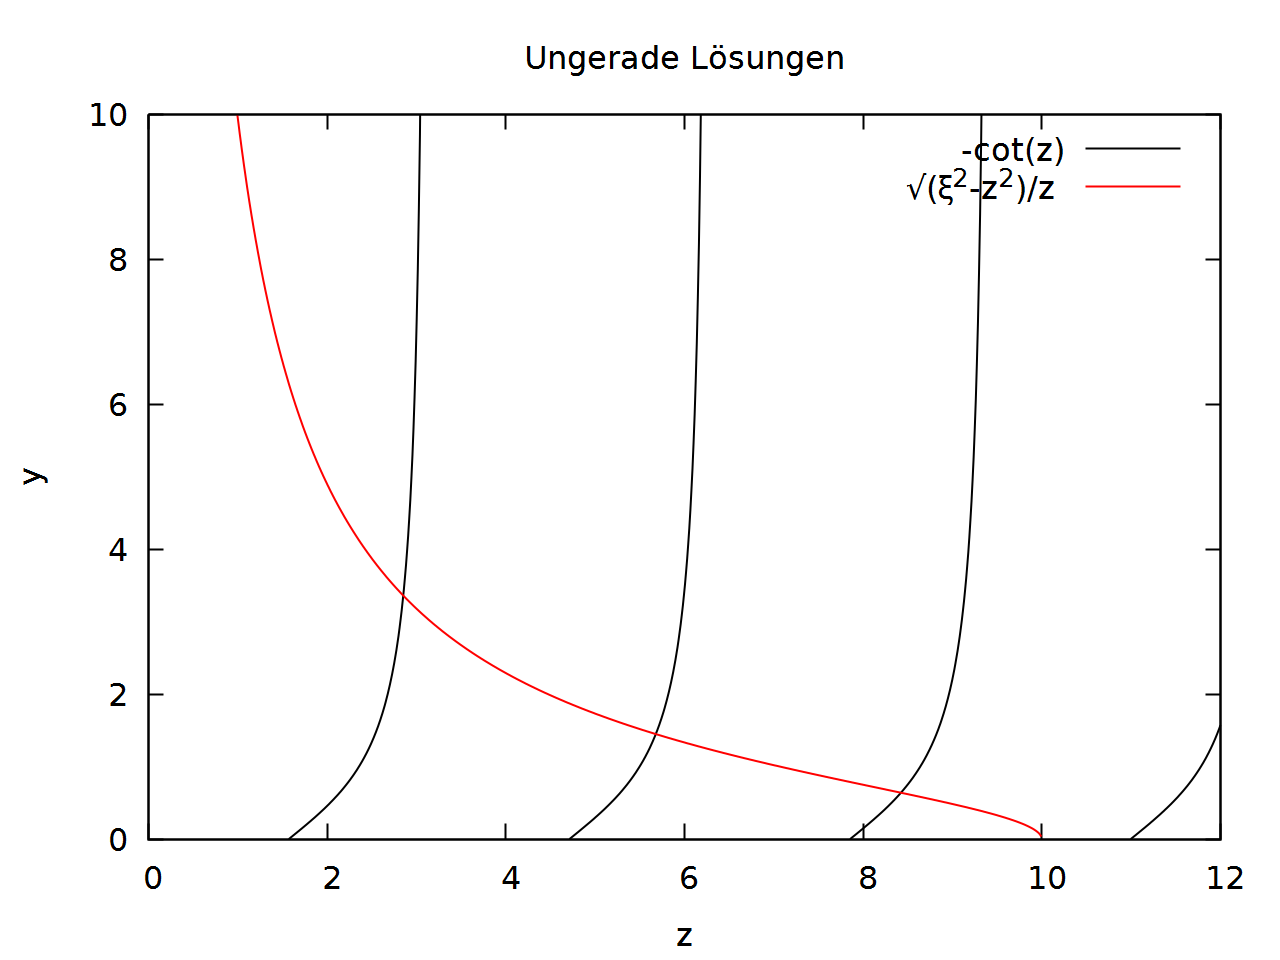
\includegraphics[scale=0.3]{plot_cot.png}
\captionof{figure}{Gerader Fall $\xi = 10$}
\end{center}

In dem Diagramm wurden sowohl $-\cot z$ als auch $\frac{\sqrt{\xi^2-z^2}}{z}$ eingezeichnet. Jeder Schnittpunkt entspricht einer Lösung. Wie man gut erkennen kann, gibt es auf jedem Arm des negativen Cotangens einen Schnittpunkt.\\

Betrachte also ein Intervall $J_k = [k\pi+\frac{\pi}{2},(k+1)\pi)$ auf dem die Funktion definiert ist, also $0 \leq (k+1)\pi < \xi$.\\
Es gilt $\lim\limits_{z\to k\pi+\frac{\pi}{2}^+}{h(z)} = \lim\limits_{z\to k\pi^+}{0 - \frac{\sqrt{\xi^2-(k\pi+\frac{\pi}{2})^2}}{k\pi+\frac{\pi}{2}}} < 0$ und $\lim\limits_{z\to (k+1)\pi-}{h(z)} = \infty > 0$. Da h(z) stetig und streng monoton steigend ist und an den Rändern verschiedene Vorzeichen hat, besitzt $h(z)$ in dem Intervall $J_k$ genau eine Nullstelle.\\

Betrachte nun das letzte Intervall $J = [k\pi+\frac{\pi}{2}, \xi)$, mit $z \leq \xi < (k+1)\pi$. Die linke Intervallgrenze hat wieder einen negativen Funktionswert, die rechte einen positiven: $\lim\limits_{z\to \xi-}{h(z)} = -\cot{\xi} - 0 > 0$.  Also gibt es auch in diesem Intervall eine Nullstelle.\\

Insgesamt gibt es somit also $n = \lfloor\frac{\xi}{\pi}-\frac{1}{2}\rfloor + 1$ Nullstellen.\\

\section*{Umsetzung}
Das gesamte Programm befindet sich in abgabe2.cpp.\\
Die Nullstellen werden mit der Bisektionsmethode ermittelt. Dazu werden immer Intervalle $[k\pi,k\pi+\pi)$ betrachtet und in dem Intervall sowohl die gerade als auch die ungerade Nullstelle berechnet. Diese werden als Liste von Paaren von (z,b) zurückgegeben, wobei das double z die Nullstelle ist, und b ein bool, der genau dann wahr ist, wenn es eine gerade Lösung ist.\\
Aufgrund des Algorithmus sind die Nullstellen schon aufsteigend in den z-Werten sortiert (und damit aufsteigend in den Energiewerten). Da es in der Aufgabenstellung verlangt war, sortieren wir die z-Werte trotzdem noch mal mit einem selbstprogrammiertem Quicksort-Algorithmus. Danach werden aus den z-Werten die Energien berechnet und diese ausgegeben. 
  

\section*{Sonstige Abgegebene Dateien}
\subsection*{plot.plt}
Die Plot-Datei für die beiden Plots in der Abgabe.

\end{document}